% =====================================================================
\section{Шина I\texorpdfstring{\textsuperscript{2}}{2}C: дисплей}
% =====================================================================
\lessonintro
  {разобраться в устройстве шины I\textsuperscript{2}C, найти устройства сканером, выводить информацию на OLED}
  {урок 2 (Serial для сканера), уроки 4--5 (состояние лампы, которое будем показывать)}
  {экран показывает, включена ли лампа и её яркость}
  {OLED-дисплей SSD1306 128×64 с интерфейсом I\textsuperscript{2}C}

\subsection{Топология шины}

I\textsuperscript{2}C использует всего два провода: \textbf{SDA} (данные) и \textbf{SCL} (такт). Выходы устройств --- с
\emph{открытым стоком}: они могут только притянуть линию к земле, а в HIGH её возвращают подтягивающие
резисторы (тот же принцип, что у кнопки в уроке 3). Каждое ведомое устройство имеет 7-битный адрес.

\begin{figure}[H]
\centering
\begin{circuitikz}[scale=0.95,transform shape]
  \draw (0,4.4) node[vcc]{3,3 В} -- (0,4.2) -- (3,4.2);
  \draw (1.5,4.2) to[R,l_=\SI{4.7}{k\ohm}] (1.5,2.8) coordinate(sdaR);
  \draw (3,4.2) to[R,l=\SI{4.7}{k\ohm}] (3,1.8) coordinate(sclR);
  \draw[thick,accent] (-1,2.8) node[left,text=accent]{SDA} -- (13,2.8);
  \draw[thick,esp] (-1,1.8) node[left,text=esp]{SCL} -- (13,1.8);
  \fill (sdaR) circle (1.5pt); \fill (sclR) circle (1.5pt);
  \node[blk,fill=blkcpu,minimum width=2.2cm,minimum height=1.2cm] (m) at (0,0) {ESP32-S3\\ \scriptsize ведущий};
  \node[blk,fill=blkper,minimum width=2.2cm,minimum height=1.2cm] (d1) at (5,0) {SSD1306\\ \scriptsize 0x3C};
  \node[blk,fill=blkper,minimum width=2.2cm,minimum height=1.2cm] (d2) at (8.2,0) {BME280\\ \scriptsize 0x76};
  \node[blk,fill=blkper,minimum width=2.2cm,minimum height=1.2cm] (d3) at (11.4,0) {…\\ \scriptsize до 112 адресов};
  \foreach \d in {m,d1,d2,d3}{
    \draw[accent] ($(\d.north)+(-0.3,0)$) -- ($(\d.north)+(-0.3,0)$ |- 0,2.8) node[circle,fill,inner sep=1.2pt]{};
    \draw[esp] ($(\d.north)+(0.3,0)$) -- ($(\d.north)+(0.3,0)$ |- 0,1.8) node[circle,fill,inner sep=1.2pt]{};
  }
  \node[font=\sffamily\scriptsize] at (0,-1) {SDA = \pin{8}, SCL = \pin{9}};
\end{circuitikz}
\caption{Шина I\textsuperscript{2}C: один ведущий, несколько ведомых на общих линиях}
\end{figure}

\begin{tip}
Большинство модулей (дисплеи, датчики на платах-переходниках) уже имеют подтягивающие резисторы. Если
на шине много модулей, суммарное сопротивление подтяжки может оказаться слишком малым --- иногда лишние
резисторы приходится выпаивать.
\end{tip}

\subsection{Временная диаграмма}

\begin{figure}[H]
\centering
\begin{tikzpicture}[x=0.72cm,y=0.8cm]
  \node[left,text=esp,font=\sffamily\small] at (0,3) {SCL};
  \draw[very thick,esp] (0,3.8) -- (2,3.8) -- (2.5,3.8) -- (2.5,2.6)
    \foreach \k in {0,...,8}{ -- ({3+\k*2},2.6) -- ({3+\k*2},3.8) -- ({4+\k*2},3.8) -- ({4+\k*2},2.6) }
    -- (21.5,2.6) -- (21.5,3.8) -- (23.5,3.8);
  \node[left,text=accent,font=\sffamily\small] at (0,1) {SDA};
  \draw[very thick,accent] (0,1.6) -- (1.2,1.6) -- (1.2,0.4) -- (2.8,0.4);
  \foreach \k/\l in {0/A6,1/A5,2/A4,3/A3,4/A2,5/A1,6/A0,7/R/W,8/ACK}{
    \pgfmathsetmacro{\xa}{2.8+\k*2}
    \draw[thick,accent] (\xa,0.4) -- (\xa+0.2,1.6) -- (\xa+1.8,1.6) -- (\xa+2,0.4);
    \draw[thick,accent] (\xa,1.6) -- (\xa+0.2,0.4) -- (\xa+1.8,0.4) -- (\xa+2,1.6);
    \node[font=\sffamily\scriptsize] at (\xa+1,1) {\l};
  }
  \draw[very thick,accent] (20.8,0.4) -- (22.3,0.4) -- (22.3,1.6) -- (23.5,1.6);
  \draw[dashed,gray] (1.2,0) -- (1.2,4.3) node[above,font=\sffamily\scriptsize,text=black]{START};
  \draw[dashed,gray] (22.3,0) -- (22.3,4.3) node[above,font=\sffamily\scriptsize,text=black]{STOP};
  \draw[decorate,decoration={brace,mirror,amplitude=4pt}] (2.8,-0.1) -- (16.8,-0.1) node[midway,below=5pt,font=\sffamily\scriptsize]{7-битный адрес (старший бит первым)};
  \draw[decorate,decoration={brace,mirror,amplitude=4pt}] (18.8,-0.1) -- (20.8,-0.1) node[midway,below=5pt,font=\sffamily\scriptsize,align=center]{ведомый\\ тянет в 0};
\end{tikzpicture}
\caption{Начало транзакции: START, адрес, бит чтения/записи, подтверждение ACK, STOP.
Данные меняются, пока SCL = LOW, и считываются, пока SCL = HIGH}
\end{figure}

\subsection{Сканер шины}

Подключите дисплей: SDA → \pin{8}, SCL → \pin{9}, питание 3V3 и GND. Первое, что стоит сделать с новым
модулем, --- убедиться, что он отвечает, и узнать его адрес.

\codecap{Сканер I\textsuperscript{2}C}
\codeinput{l6_scanner}

\subsection{Первый вывод на экран}

Установите через \textsf{Library Manager} библиотеки \textbf{Adafruit SSD1306} и \textbf{Adafruit GFX}.
Библиотека рисует в буфере в памяти, а \code{display()} отправляет весь буфер (1 КБ) по шине.

\codecap{Hello на OLED-дисплее}
\codeinput{l6_oled_hello}

\begin{tip}
Стандартные шрифты Adafruit GFX не содержат кириллицы --- для русского текста нужны сторонние шрифты
или библиотека U8g2 с кириллическими наборами. В проекте обойдёмся латиницей.
\end{tip}

\subsection{Шаг проекта 6: экран состояния}

\progress{6}

\begin{figure}[H]
\centering
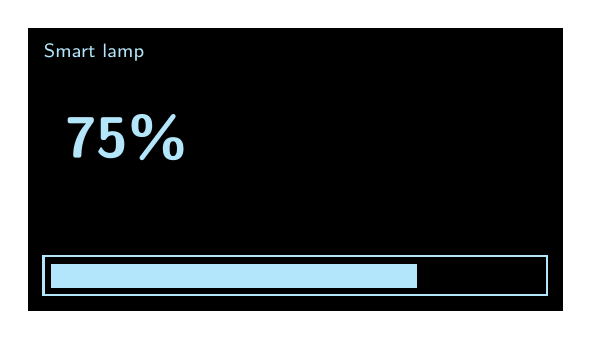
\begin{tikzpicture}[x=0.5mm,y=-0.5mm]
  \fill[black] (-4,-4) rectangle (132,68);
  \node[anchor=north west,font=\sffamily\scriptsize,text=cyan!30,inner sep=0] at (0,0) {Smart lamp};
  \node[anchor=north west,font=\sffamily\bfseries\huge,text=cyan!30,inner sep=0] at (0,18) {~75\%};
  \draw[cyan!30,thick] (0,54) rectangle (128,64);
  \fill[cyan!30] (2,56) rectangle (95,62);
\end{tikzpicture}
\caption{Экран лампы: заголовок, яркость крупно и полоска-индикатор}
\end{figure}

Рисовать экран в каждом проходе \code{loop()} не нужно: отправка буфера занимает десятки
миллисекунд. Обновляем его 10 раз в секунду --- тем же приёмом с \code{millis()}, что и «пульс».

\codecap{Умная лампа, шаг 6 (изменения относительно шага 5)}
\codeinput{lamp_step6}

Лампа готова как автономное устройство. Но посмотрите на \code{loop()}: в нём уже пять разных дел,
и каждое вынуждено «уступать» остальным. Пока отправляется буфер экрана, кнопка не опрашивается;
добавь сюда ещё и сеть --- и разобраться, кто кому мешает, станет трудно. Эту проблему решает следующий урок.

\begin{summary}
\begin{itemize}[leftmargin=*]
  \item I\textsuperscript{2}C --- два провода, подтяжки, адреса; первым делом запускайте сканер.
  \item Библиотека дисплея рисует в буфере; \code{display()} отправляет его целиком --- это небыстро.
  \item Медленные действия выполняем периодически, а не на каждом проходе \code{loop()}.
\end{itemize}
\end{summary}

\begin{tasks}
\begin{enumerate}
  \item Добавьте датчик BME280/AHT20 на ту же шину и показывайте температуру в заголовке экрана.
  \item Нарисуйте график изменения яркости за последние 128 обновлений экрана.
  \item Сделайте «заставку»: через 10 с без действий экран тускнеет (\code{display.dim(true)}).
\end{enumerate}
\end{tasks}
